% 
\documentclass[11pt]{article}
\usepackage{amscd,amsfonts,amssymb,amstext,latexsym} 
\usepackage{amsmath,mathbbol,mathrsfs,stmaryrd, mathtools} 
%\usepackage{mathbbol,mathrsfs,stmaryrd}
\usepackage {algorithm2e} 
\usepackage{theoremref}
\usepackage[T1]{fontenc}
\usepackage[english]{babel} 
\usepackage {enumerate}
\usepackage{url}
%\usepackage {algpseudocode}  
\usepackage{graphics} 
\usepackage{tikz}
\usepackage[square]{natbib}
\usepackage[width=14.8cm,left=3cm]{geometry}
\usetikzlibrary{automata,calc}
%\usepackage{tgtermes} 
\usepackage{listings}

\usepackage{color} %red, green, blue, yellow, cyan, magenta, black, white
\definecolor{mygreen}{RGB}{28,172,0} % color values Red, Green, Blue
\definecolor{mylilas}{RGB}{170,55,241}
\usepackage{subfig}

\usepackage{mathptmx}
\usepackage{fancyhdr}
\usepackage{verbatim}
\usepackage{enumitem}
\usepackage{booktabs}
\usepackage[flushleft]{threeparttable}
\usepackage{listings}
\usepackage{verbatim}
\usepackage{fancyhdr}
\usepackage{multirow,multicol}
\usepackage[colorlinks=true,linkcolor=blue,citecolor=blue,urlcolor=blue]{hyperref}
\usepackage{tabto}
\usepackage{float} %added for image location
\lstset{ %
language=C++,                % choose the language of the code
basicstyle={\ttfamily},       % the size of the fonts that are used for the code
backgroundcolor=\color{white},  % choose the background color. You must add \usepackage{color}
showspaces=false,               % show spaces adding particular underscores
aboveskip=6mm, 
%belowskip=3mm, 
numbers=left, numberfirstline=false, numberblanklines=false,
numberstyle=\tiny\color{gray}, numbersep= 5pt, 
showstringspaces=false,         % underline spaces within strings
showtabs=false,                 % show tabs within strings adding particular underscores
%frame=single,           % adds a frame around the code
%frame = tb, 
frame = none, 
tabsize=2,          % sets default tabsize to 2 spaces
captionpos=b,           % sets the caption-position to bottom
breaklines=true,        % sets automatic line breaking
breakatwhitespace=false,    % sets if automatic breaks should only happen at whitespace
escapeinside={\%*}{*)}          % if you want to add a comment within your code
}
\graphicspath{{./results/}}
\fancypagestyle{plain}{
\fancyhf{}
\rhead{School of Computer Science and Applied Mathematics\\ 
%\noindent\rule{15.4cm}{0.4pt}\\
\footnotesize{\textsc{University of the Witwatersrand, Johannesburg}}}
\lhead{
\includegraphics[scale=0.08]{witslogo_h.png}}
\fancyfoot[C]{\thepage}
\renewcommand{\headrulewidth}{0.4pt}
}

\textwidth=16.8cm 
\textheight=20cm  % change this to adjust the height and bottom margin of the doc
\evensidemargin 0pt 
\oddsidemargin 0pt 
\leftmargin 0pt 
\rightmargin 0pt 
\setlength{\topmargin}{0pt} 
\setlength{\footskip}{50pt}
\setlength{\parindent}{0pt}
\setlength{\parskip}{1em}
\linespread{1} 
% 
\makeatletter
\newcommand{\rmnum}[1]{\romannumeral #1}
\newcommand{\Rmnum}[1]{\expandafter\@slowromancap\romannumeral #1@}
\makeatother


\begin{document}
\title{COMS4040A \& COMS7045A Assignment 3 -- Report}
\author{Abdulkadir Dere - 752817 - Computer Science Hons}
\date{29 May 2020} 
\maketitle 
%\thispagestyle{empty}
\pagestyle{fancy}
\fancyhf{}
\fancyhead[R]{\thepage}
\fancyhead[L]{COMS4040A \& COMS7045A Assignment 3}
%\vskip 3mm 
%\pagenumbering{roman}
%\newpage



\lstset{language=C,%
    basicstyle=\ttfamily,
    frame=single,
    breaklines=true,%
    % belowskip=3em,
    morekeywords={matlab2tikz},
    keywordstyle=\color{blue},%
    morekeywords=[2]{1}, keywordstyle=[2]{\color{black}},
    identifierstyle=\color{black},%
    stringstyle=\color{mylilas},
    commentstyle=\color{mygreen},%
    showstringspaces=false,%without this there will be a symbol in the places where there is a space
    numbers=left,%
    numberstyle={\tiny \color{black}},% size of the numbers
    numbersep=9pt, % this defines how far the numbers are from the text
    % emph=[1]{for,end,break},emphstyle=[1]\color{red}, %some words to emphasise
    emph=[1]{serial_convolution, global_convolution, shared_convolution, convolution, applyMask, neighbours, },emphstyle=[1]\color{red}, %some words to emphasise
    %emph=[2]{word1,word2}, emphstyle=[2]{style},    
}


\section{Introduction} 
In this report, we will focus on the different design methodologies used to create 2D convolution on provided images. We will look at serial implementation, CUDA implementation using both global memory and constant memory, CUDA implementation using both shared memory and constant memory and CUDA implementation using texture memory. Each design methodology is defined and process has been explained with the code.

\section{Methodology}
We will be using averaging, edge detection and sharpening masks for the convolution process.

\begin{table}[]
\centering
\begin{tabular}{|l|l|l|}
\hline
-1 & -1 & -1 \\ \hline
-1 & 9  & -1 \\ \hline
-1 & -1 & -1 \\ \hline
\end{tabular}
\hspace{0.5cm}
\begin{tabular}{|l|l|l|}
\hline
-1 & 0 & 1 \\ \hline
-2 & 0  & 2 \\ \hline
-1 & 0 & 1 \\ \hline
\end{tabular}
\hspace{0.5cm}
\begin{tabular}{|l|l|l|}
\hline
1 & 1 & 1 \\ \hline
1 & 1  & 1 \\ \hline
1 & 1 & 1 \\ \hline
\end{tabular}
\caption{Masks used for convolution: sharpening, edge detection and averaging respectively}
\label{tab:my-table}
\end{table}

\subsection{Serial Computation}
We will first implement the serial version of 2D image convolution algorithm using the CPU. Serial version of the algorithm will follow the following design methodology:
\begin{itemize}[leftmargin=0em]
%\setlength\itemsep{-0.2em}
  \setlength{\itemsep}{0pt}
  \item Read the image using built-in functions. 2D image is returned as 1D image and assigned to a variable.
  \item Convert the read image from 1D to 2D for easier computation of convolution algorithm since the image is in 2D.
  \item Pad the image so mask we can compute the corners of the image. Image will be padded with zero padding. 
  \item Apply the convolution mask/filter to the padded image. The convolution algorithm will be executed as a recursive algorithm. The process will start by selecting the first element of the array excluding the padded pixels. We will subtract padded size from offset (half size of the mask) to find the starting row and column of the image. This pixel must be same as the original pixel. We will apply the convolution mask to this pixel. (Algorithm \ref{lst: serial_convolution})
  \item The convolution mask application process starts by identifying the neighbours of the given pixel location. We will compute neighbours according to the mask size since image will be padded by the factor of half of mask on all four sides. We will not run out-of-bounds when retrieving the pixel values for each neighbour since the image is padded. We will create a convolution results array with the dimensions of the mask size to compute the results. We will do element-wise multiplication between neighbours and the mask. All of these values will be added together to compute the convolution result of the given pixel location. (Algorithm \ref{lst: applyMask})
  \item The convolution result for the pixel location will be saved in the output image and process will continue with the next pixel location until algorithm iterates through all the pixels. (Algorithm \ref{lst: serial_convolution})
  \item The padded area will be removed by un-padding the padded image to retrieve the results in original image dimensions.
  \item The resulting image will be converted from 2D array to 1D to save the resulting convolution image. 
\end{itemize}

The code for the detailed methodology has been provided with comments. Pre-processing and post-processing functions are not included in the report. These functions can be founds in the following file: $serialConvolution.cu$ under $src$ folder.

\begin{lstlisting}[language=C, label={lst: serial_convolution}, caption= Add zero padding to the image]
// 2D serial convolution method
double **serial_convolution(double **input, double **output){
    int range = padded_size - offset;
    // printf("range: %d \n", range);

    for (int i = offset; i<range; i++){
        for (int j = offset; j<range; j++){
            output[i][j] = applyMask(input, i, j);
        }
    }
    return output;
}
\end{lstlisting}

\begin{lstlisting}[language=C, label={lst: applyMask}, caption= Apply convolution mask to the given pixel]
double applyMask(double **array, int row, int col){
    int n_size = offset * 2 + 1;

    // neighbours of given location
    double **neighbours = allocateMatrix(n_size, n_size);

    // dynamically get the neighbours range
    int n1 = 0;
    for (int r=row - 1; r <= row + offset; r++){
        int n2 = 0;
        for (int c =col - 1; c <= col + offset; c++){
            neighbours[n1][n2] = array[r][c];
            n2++;
        }
        n1++;
    }
    
    double **convolution = allocateMatrix(n_size, n_size);
    double value = 0;
    for (int r=0; r<3; r++){
        for(int c=0; c<3; c++){
            convolution[r][c] = mask[r][c] * neighbours[r][c];
            value = value + convolution[r][c];
        }
    }
    return value;
}
\end{lstlisting}


\subsection{CUDA implementation using both global memory and constant memory}
Image convolution using CUDA C has been implemented using both global memory and constant memory. The convolution mask is constant through out the convolution process. It is beneficial to cache the convolution mask in the constant memory as this informs the CUDA runtime that mask values will not change during kernel execution (\cite{parallel}) (Algorithm \ref{lst: mask_global}). The constant memory will set the mask value as read-only and it will be broadcasted to all elements in the convolution kernel execution. The convolution process will be done in global memory using a CUDA kernel (Algorithm \ref{lst: global_convolution}). The kernel parameters consist of original image, allocated space for resulting image, width and height of the original image. The row and column indexes will be computed to identify which index will be computed by which thread. The starting index for row and column will be calculated by subtracting the offset value because we want to ignore the padded area. This will let the convolution process to start and end at dimensions of the original image so we don't run out-of-bounds. The kernel will calculate each convolution value by calculating all the elements within the mask filter size (dimension) and add all of them to get the convolution value for a specific pixel. The row and column indexes will be verified so that we are within the dimensions. The resulting value will be saved to the resulting image space.


\begin{lstlisting}[language=C, label={lst: mask_global}, caption= Cache mask in to the constant memory]
// Convolution Mask Dimension
#define MASK_DIM 3
#define OFFSET (MASK_DIM/2)

// allocate mask in constant memory
__constant__ float d_mask_global[MASK_DIM * MASK_DIM];
\end{lstlisting}


\begin{lstlisting}[language=C, label={lst: global_convolution}, caption= 2D Convolution using the global memory]
// 2D convolution using global and constant memory
__global__ void global_convolution(float *d_Data, float *d_result, int width, int height) {
  // calculate the row and column index to compute for each thread
  int row = blockIdx.y * blockDim.y + threadIdx.y;
  int col = blockIdx.x * blockDim.x + threadIdx.x;

  // Starting index for convolution so we can ignore the padded area
  int i_row = row - OFFSET;
  int i_col = col - OFFSET;

  // convolution value to be calculated for each pixel's row and column
  double value = 0;
  // iterate over all rows and column using the mask dimension.
  // this will calculate all the neighbours and origin pixel and sum these values to give
  // us the value of the origin pixel
  for (int i = 0; i < MASK_DIM; i++) {
    for (int j = 0; j < MASK_DIM; j++) {
      if ((i_row + i) >= 0 && (i_row + i) < height && (i_col + j) >= 0 && (i_col + j) < width) {
      	// sum all the values within the range of the mask to get origin pixel's value
           value += d_Data[(i_row + i) * width + (i_col + j)] * d_mask_global[i * MASK_DIM + j];
      }
    }
  }
  // write back convolution result
  d_result[row * width + col] = value;
}
\end{lstlisting}


\subsection{CUDA implementation using both shared memory and constant memory}
In this section, we will look at image convolution using both shared memory and constant memory.

\begin{lstlisting}[language=C, label={lst: mask_shared}, caption= Cache mask in to the constant memory]
// Convolution Mask Dimension
#define MASK_DIM 3
#define OFFSET (MASK_DIM/2)

#define TILE_WIDTH 16
#define RADIUS 2
#define BLOCK_WIDTH (TILE_WIDTH+(2*RADIUS))

#define DIAMETER (RADIUS*2+1) // mask diameter
#define SIZE (RADIUS*DIAMETER) // mask size

// allocate mask in constant memory
__constant__ float d_mask_shared[MASK_DIM * MASK_DIM];
\end{lstlisting}


\begin{lstlisting}[language=C, label={lst: shared_convolution}, caption= 2D Convolution using the shared memory]
__global__ void shared_convolution(float* dData, float* dResult, unsigned int width, unsigned int height){

  // create tile in shared memrory for the convolution
  __shared__ float shared[BLOCK_WIDTH * BLOCK_WIDTH];

    // for simplicity to use threadIdx
    int tx = threadIdx.x;
    int ty = threadIdx.y;
    int bx = blockIdx.x;
    int by = blockIdx.y;

    // get row and column index of pixels in the tile
    int col = bx * TILE_WIDTH + tx - RADIUS;
    int row = by * TILE_WIDTH + ty - RADIUS;

    // Find the last and first pixel locations within the image
    col = max(0, col);
    col = min(col, width-1);
    row = max(row, 0);
    row = min(row, height-1);

    // load the tile pixels from the global memory into shared memory
    // this will help us to reduce global memory access by the factor of 1/TILE_WIDTH
    // ignore any pixels which are out-of-bounds (i.e. padded area)
    unsigned int index = row * width + col;
    unsigned int block_index = ty * blockDim.y + tx;
    shared[block_index] = dData[index];

    // thread barrier to wait for all the threads to finish loading from
    // global memory to shared memory
    __syncthreads();
  
    // Elementwise multiplication of pixel and mask values and add all of the values within the mask
    // range to get output value of one pixel. Verify that we are not working out-of-bounds of the image
    // We will iterate over rows and columns within the mask dimensions (i.e. all the neighbours)
    float value = 0;
    if (((tx >= RADIUS) && (tx < BLOCK_WIDTH-RADIUS)) && ((ty>=RADIUS) && (ty<=BLOCK_WIDTH-RADIUS))){
      for(int i = 0; i<MASK_DIM; i++){
          for(int j = 0; j<MASK_DIM; j++){ 
            value += shared[block_index+(i*blockDim.x)+j] * d_mask_shared[i*3+j];
          }
      }
      dResult[index] = value;
  }
}\end{lstlisting}


\section{Questions and Answers}



\section{Experiment} 
\subsection{Experiment Setup}
Experiments are conducted on a cluster. The details for the CUDA device are listed.\\
CUDA Device 0\\
Major revision number:         6\\
Minor revision number:         1\\
Name:                          GeForce GTX 1060 6GB \\ 
Total global memory:           6371475456 \\
Total shared memory per block: 49152 \\
Total registers per block:     65536 \\
Warp size:                     32 \\ 
Maximum memory pitch:          2147483647 \\
Maximum threads per block:     1024 \\
Maximum dimension 0 of block:  1024 \\
Maximum dimension 1 of block:  1024 \\
Maximum dimension 2 of block:  64 \\
Maximum dimension 0 of grid:   2147483647 \\
Maximum dimension 1 of grid:   65535 \\
Maximum dimension 2 of grid:   65535 \\
Clock rate:                    1784500 \\
Total constant memory:         65536 \\
Texture alignment:             512 \\
Concurrent copy and execution: Yes \\
Number of multiprocessors:     10 \\
Kernel execution timeout:      Yes \\

\subsection{Experiment Results}
Experimental results are shown with different distance and sorting algorithms and with varying $n$ query points.

\begin{table}[]
\centering
\begin{tabular}{|l|c|c|}
\hline
\textbf{Image}                                                                                           & \textbf{image21.pgm} & \textbf{lena\_bw.pgm} \\ \hline
\textbf{Matrix Size}                                                                                     & 512x512              & 512x512               \\ \hline
\textbf{Tile Size}                                                                                       & 16x16                & 16x16                 \\ \hline
\textbf{\begin{tabular}[c]{@{}l@{}}Serial Convolution\\ Time (ms)\end{tabular}}                          & 154.862244           & 152.380386            \\ \hline
\textbf{\begin{tabular}[c]{@{}l@{}}Global Memory\\ Time (ms)\end{tabular}}                               & 0.093184             & 0.094880              \\ \hline
\textbf{\begin{tabular}[c]{@{}l@{}}Shared Memory \\ Time (ms)\end{tabular}}                              & 0.030656             & 0.032704              \\ \hline
\textbf{\begin{tabular}[c]{@{}l@{}}Speedup of global memory\\ kernel (ms)\end{tabular}}                  & 1661.9               & 1606.03               \\ \hline
\textbf{\begin{tabular}[c]{@{}l@{}}Speedup of shared memory\\ kernel (ms)\end{tabular}}                  & 5051.61              & 4659.38               \\ \hline
\textbf{\begin{tabular}[c]{@{}l@{}}Throughput of serial\\ implementation (GFLOPS)\end{tabular}}          & 0.0152348            & 0.0154829             \\ \hline
\textbf{\begin{tabular}[c]{@{}l@{}}Throughput of global\\ memory implementation\\ (GFLOPS)\end{tabular}} & 25.3187              & 24.8661               \\ \hline
\textbf{\begin{tabular}[c]{@{}l@{}}Throughput of shared\\ memory implementation\\ (GFLOPS)\end{tabular}} & 76.9603              & 72.1409               \\ \hline
\textbf{\begin{tabular}[c]{@{}l@{}}Performance improvement: \\ global over serial\end{tabular}}          & 1661.9x              & 1606.03x              \\ \hline
\textbf{\begin{tabular}[c]{@{}l@{}}Performance improvement: \\ shared over serial\end{tabular}}          & 5051.61x             & 4659.38x              \\ \hline
\textbf{\begin{tabular}[c]{@{}l@{}}Performance improvement: \\ shared over global\end{tabular}}          & 3.03967x             & 2.90117x              \\ \hline
\end{tabular}
\caption{Results of the convolutions applied to the given images.}
\label{tab:results-table}
\end{table}



\begin{figure}[H]
\centering
\subfloat[]{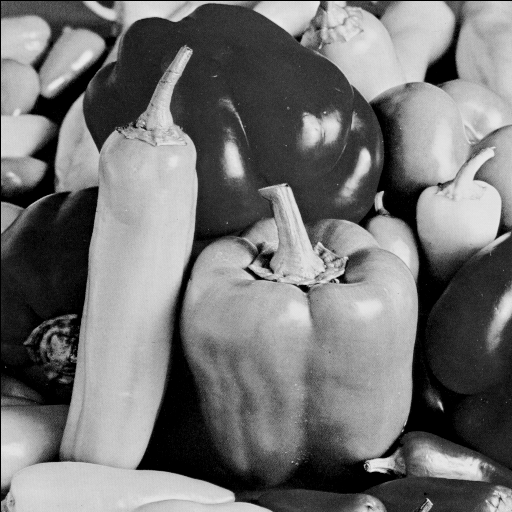
\includegraphics[width=.2\textwidth]{image21.png}} \hfill
\subfloat[]{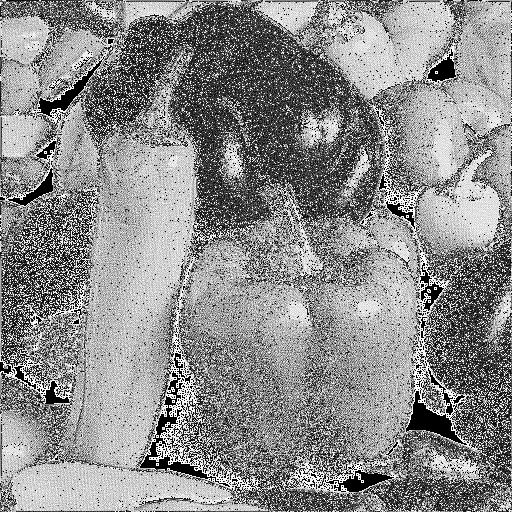
\includegraphics[width=.2\textwidth]{image21_sharpening.png}} \hfill
\subfloat[]{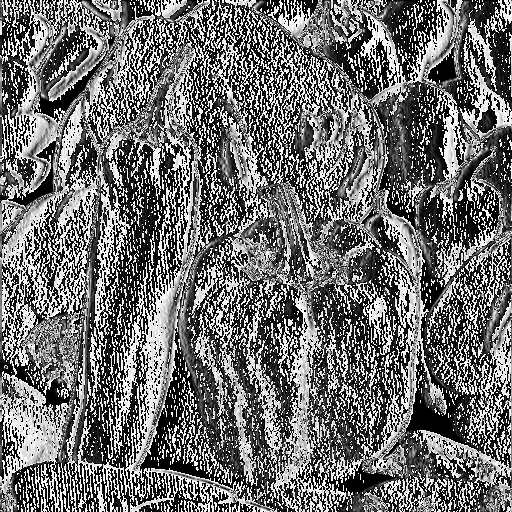
\includegraphics[width=.2\textwidth]{image21_edge.png}} \hfill
\subfloat[]{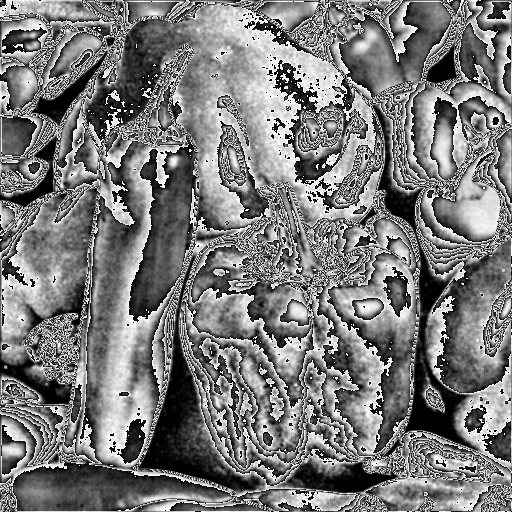
\includegraphics[width=.2\textwidth]{image21_averaging.png}} \hfill
\caption{Convolution results for the $image21$ image (a) Original Image (b) Sharpening (c) Edge detection (d) Averaging}
\label{fig:image21}
\end{figure}

\begin{figure}[H]
\centering
\subfloat[]{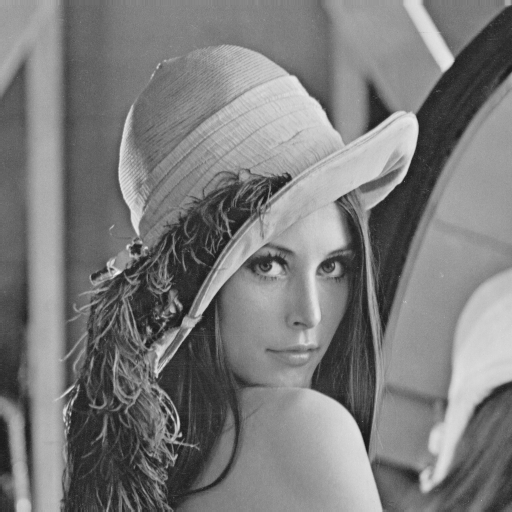
\includegraphics[width=.2\textwidth]{lena_bw.png}} \hfill
\subfloat[]{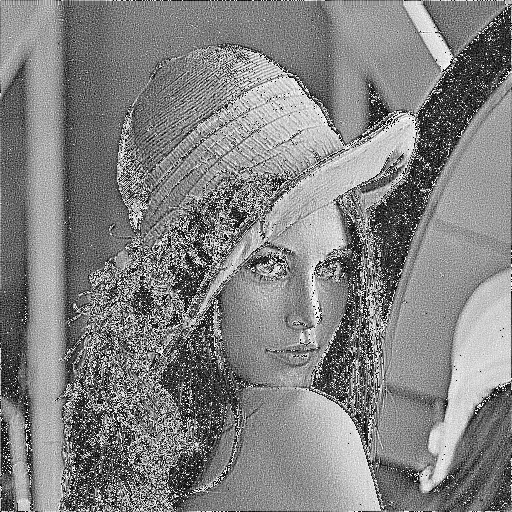
\includegraphics[width=.2\textwidth]{lena_bw_global_sharpening.png}} \hfill
\subfloat[]{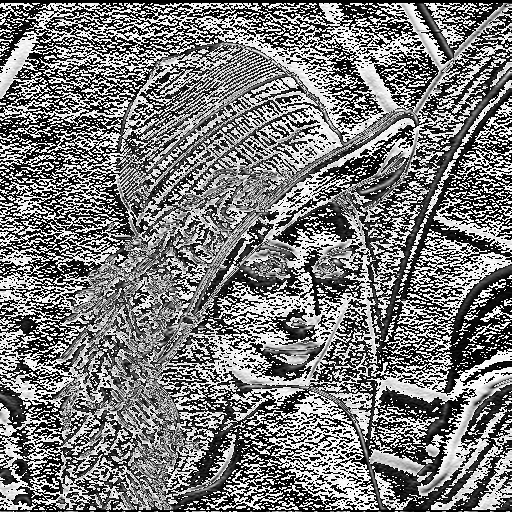
\includegraphics[width=.2\textwidth]{lena_bw_shared_edge.png}} \hfill
\subfloat[]{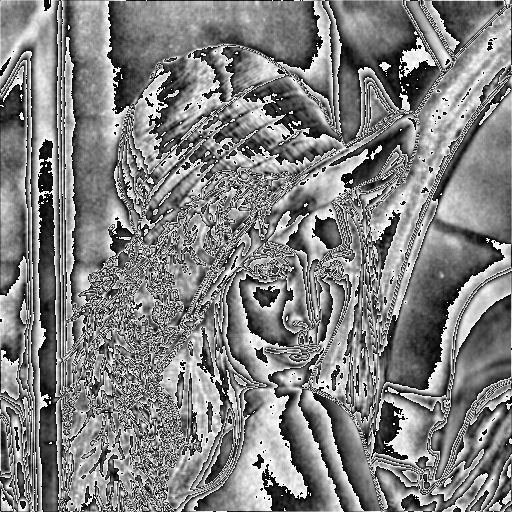
\includegraphics[width=.2\textwidth]{lena_bw_averaging.png}} \hfill
\caption{Convolution results for the $lena\_bw$ image (a) Original Image (b) Sharpening (c) Edge detection (d) Averaging}
\label{fig:lena}
\end{figure}


\subsection{Summary of Results}
As we can see from the Table~\ref{tab:results-table} that global memory version has greatly improved on the serial implementation. The shared memory version has improved on global memory and serial implementations. However, global memory implementation is still not at its top efficiency since every thread calculates its own output. This can be increased by implementing threads to compute a tile of the image similar to shared memory implementation. 

\section{Conclusion} 


\newpage
\bibliographystyle{apalike}
\bibliography{bibfile}

\pagenumbering{arabic} 
\end{document} 




%\bibliographystyle{apalike}
%\bibliography{bibfile}
%\bibliography{../HPC}


